\chapter{Raytracing}
\section{Grundidee}
Raytracing erzeugt fotorealistische Bilder, indem es Spiegelung und Transparenz berechnet. Grundsätzlich generiert man für jeden Pixel eine Linie in das Bild hinein und schaut dann, welches Objekt diese Linie zuerst schneidet. Wenn das erste Objekt gefunden wurde, dann berechne die Farbe. Simpel as that.
\begin{figure}[!ht]
	\centering
	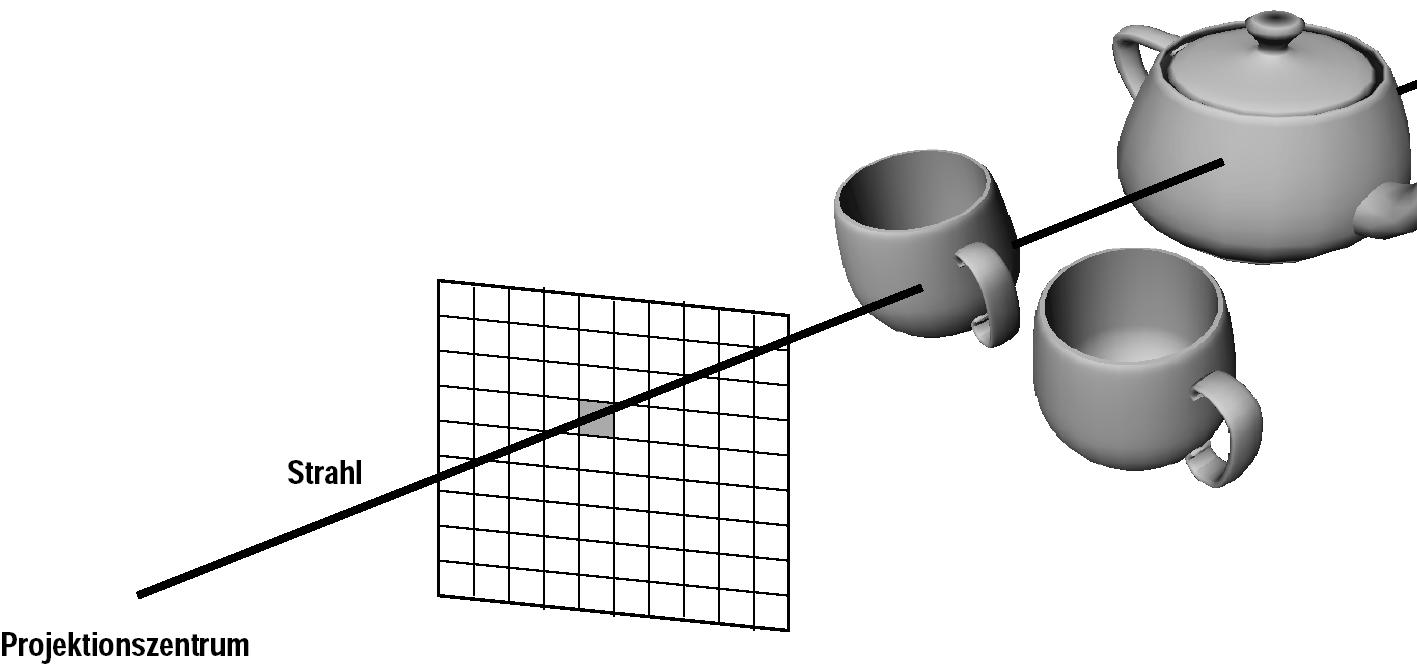
\includegraphics[width=0.4\linewidth]{fig/raytracing}
	\caption{Raytracing Grundidee}
	\label{fig:raytracing}
\end{figure}

\section{Rekursives Raytracing}
Mit dem ersten Strahl auf das Objekt ist noch nicht viel Realität in den PC geholt worden. Erst mit dem rekursiven Raytracing kommt das.

\begin{figure}[!ht]
	\centering
	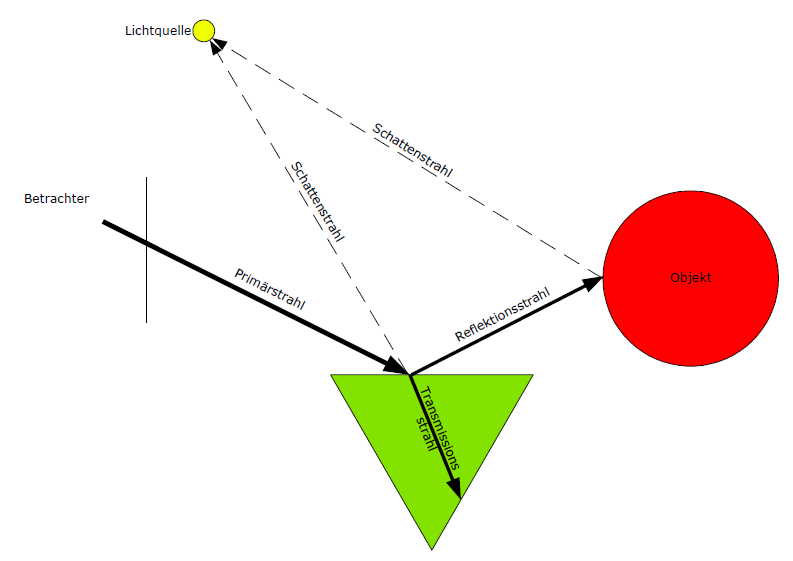
\includegraphics[width=0.5\linewidth]{fig/raytracing_rekursiv}
	\caption{Rekursives Raytracing}
	\label{fig:raytracing_rekursiv}
\end{figure}

Wir haben also den ersten Strahl vom Betrachter aus - unseren \textit{Primärstrahl}. Dieser geht vom Betrachter direkt auf den betrachteten Pixel. Von dort aus machen wir weitere Strahlen - einmal ein Reflexionsstrahl, der ähnlich wie der Primärstrahl einfach das nächste Objekt sucht und schaut, was dort für eine Farbe ist und diese dann dem ersten Punkt hinzufügt. Dann gibt es noch die Schattenstrahlen, die von der Lichtquelle aus berechnen, wie sehr diese jetzt den Punkt beleuchten. Dann gibt es no den Transmissionsstrahl, der durch das Objekt hindurch geht, und die Farbe holt, die am anderen Ende des Objekts ist. Wir haben also:
\begin{enumerate}
	\item \textbf{Primärstrahl} - Der erste Strahl vom Betrachter zum Objekt
	\item \textbf{Schattenstrahl} - Der Strahl vom betracheten Punkt zur Lichtquelle
	\item \textbf{Reflektionsstrahl} - Der Strahl der Reflektion
	\item \textbf{Transmissionsstrahl} - Der Strahl der durch das Objekt hindurch geht
\end{enumerate}

Jetzt kommt es natürlich nur noch darauf an, wie tief man diese Strahlen verfolgt. Irgendwann sind sie nur noch so schwach, dass sie fast keinen Einfluss mehr darauf haben, wie das Bild aussieht, deswegen hört man auch irgendwann auf - und auch natürlich wegen der Rechenzeit ist es wichtig, diese \textit{Strahlentiefe} zu begrenzen.

\subsection{Aliasing}
Weil man nicht so schöne Bilder erhält mit dem Raytracing an sich, verwendet man noch ein adaptives Supersampling. Man macht also bis zu 16 Rays pro Pixel und fügt diese dann zu einem Pixel wieder zusammen.

\chapter{Radiosity}
Wir verwenden ein globales Beleuchtungsmodell für die korrekte diffuse Beleuchtung. Wichtig so für Architektur oder Industriedesign - da sollte es irgendwie realistisch aussehen. Das ganze nennt sich auch \textit{Global Illumination}. Man unterscheidet hier nicht zwischen Leuchtquellen und beleuchteten Flächen - weil diese ja auch wieder reflektieren. Es ist also eigentlich ein geschlossenes System aus Sicht der Energieerhaltung. Im Gegensatz zu Raytracing wird hier das gesamte Modell schon einmal vorberechnet und beleuchtet, sodass der Betrachtungsstandort dann schlussendlich egal ist.
\section{Detailkonzept}
Wir haben ja verschiedene Objekte. Wir unterteilen jetzt diese Oberflächen in \textit{Patches}. Ein Patch hat immer dieselbe Lichtintensität - ist also im Prinzip ein 'Licht-Pixel' irgendwie. Der Leuchtet dann auf andere Patches und andere Patches leuchten auf ihn. Das Ganze modellieren wir mit Hilfe von linearen Gleichungen. Da wir diese Gleichungen nie im Detail angeschaut haben, werde ich sie hier mal nicht aufführen. Wir könnten Gleichungssysteme aber mit diesen Verfahren lösen:
\begin{enumerate}
	\item Jacobi Iteration
	\item Gauss Seidel Relaxation
	\item Southwell Iteration
\end{enumerate}
Ist aber grundsätzlich sehr Aufwändig so ein Global Illumination Modell zu berechnen. Vorallem der Austausch zwischen den Patches, der sog. \textit{Formfaktor} ist am schwierigsten, z.B. hat er ein Doppelintegral und alles. Zudem muss zwischen jedem Patch berechnet werden, ob sie überhaupt untereinander sichtbar sind, wie viel Licht da ausgetaucht wird (Winkel usw), ... Deswegen nimmt man dort häufig geometrische Approximationen vom Ganzen, also z.B. mit Halbkugeln oder würfeln.

\section{Optimierungen}
\subsection{Progressive Radiosity}
Man zeigt schon früh einmal ein approximatives Resultat des Bildes und berechnet dann immer weiter die Details.
\subsection{Hierarchical Radiosity}
Die Patches zu verteilen ist ja sehr schwierig - macht man zu viele hat man zu lange zum Berechnen, zu wenig und es sieht doof aus. Also macht man hierarchical radiosity und nimmt einfach dort, wo es nötig ist ein paar mehr patches und sonst nicht. Es ist eher nötig, wenn viel Licht ausgetauscht wird oder die Patches nahe beieinander sind.